\documentclass{standalone}    
\usepackage{catchfilebetweentags}
\usepackage{amssymb}
\usepackage{turnstile}
\usepackage{bbm}
\usepackage[greek, english]{babel}
\usepackage{MnSymbol}
\usepackage{csquotes}
\newcommand\doubleplus{+\kern-1.3ex+\kern0.8ex}
\newcommand\mdoubleplus{\ensuremath{\mathbin{+\mkern-8mu+}}}
\makeatletter
\newcommand\incircbin
{%
  \mathpalette\@incircbin
}
\newcommand\@incircbin[2]
{%
  \mathbin%
  {%
    \ooalign{\hidewidth$#1#2$\hidewidth\crcr$#1\bigcirc$}%
  }%
}
\newcommand{\oeq}{\ensuremath{\incircbin{=}}}
\makeatother
\usepackage{ucs}
\DeclareUnicodeCharacter{8759}{\ensuremath{\squaredots}}
\DeclareUnicodeCharacter{951}{\textgreek{\texteta}}
\DeclareUnicodeCharacter{737}{\ensuremath{^\text{l}}}
\DeclareUnicodeCharacter{691}{\ensuremath{^\text{r}}}
\DeclareUnicodeCharacter{7523}{\ensuremath{_\text{r}}}
\DeclareUnicodeCharacter{8718}{\ensuremath{\blacksquare}}
\DeclareUnicodeCharacter{957}{\textgreek{\textnu}}
\DeclareUnicodeCharacter{961}{\textgreek{\textrho}}
\DeclareUnicodeCharacter{929}{\textgreek{\textRho}}
\DeclareUnicodeCharacter{954}{\textgreek{\textkappa}}
\DeclareUnicodeCharacter{10214}{\ensuremath{\lsem}}
\DeclareUnicodeCharacter{10215}{\ensuremath{\rsem}}
\DeclareUnicodeCharacter{8857}{\mdoubleplus}
\DeclareUnicodeCharacter{8860}{\oeq}
\DeclareUnicodeCharacter{9043}{\ensuremath{\triangle}}
\DeclareUnicodeCharacter{928}{\textgreek{\textPi}}
\DeclareUnicodeCharacter{922}{\textgreek{\textKappa}}
\DeclareUnicodeCharacter{931}{\textgreek{\textSigma}}
\DeclareUnicodeCharacter{916}{\textgreek{\textDelta}}
\DeclareUnicodeCharacter{8779}{\ensuremath{\backtriplesim}}
\usepackage[utf8x]{inputenc}
\usepackage[T1]{fontenc}
\usepackage{autofe}
\usepackage[references]{agda}
\usepackage{bbding}
\usepackage{tikz}
\usetikzlibrary{decorations.pathmorphing}
\usetikzlibrary{snakes}
\usetikzlibrary{arrows}
\usetikzlibrary{cd}

\begin{document} 
    \begin{tikzpicture}
      % \draw[help lines] (-8,-4) grid (8,3); 
      \node (ln) at (-2, 2) {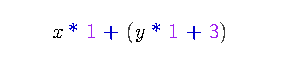
\includegraphics[draft=false,trim={25 10 35 10}]{rhs-norm}};
      \node (rn) at ( 2, 2) {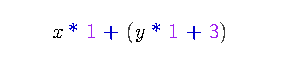
\includegraphics[draft=false,trim={25 10 35 10}]{rhs-norm}};
      \node (la) at (-6, 0) {
\includegraphics[draft=false,trim={25 10 22 10}]{lhs-ast}};
      \node (ra) at ( 6, 0) {
\includegraphics[draft=false,trim={25 10 25 10}]{rhs-ast}};
      \node (le) at (-2,-2) {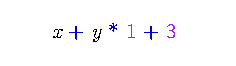
\includegraphics[draft=false,trim={25 10 23 10}]{lhs-expr}};
      \node (re) at ( 2,-2) {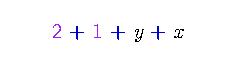
\includegraphics[draft=false,trim={25 10 25 10}]{rhs-expr}};
      \draw[|-stealth] (la) to[out=90 , in=180] node[midway, fill=white] {\AgdaFunction{⟦\_⇓⟧}} (ln);
      \draw[|-stealth] (la) to[out=270, in=180] node[midway, fill=white] {\AgdaFunction{⟦\_⟧} } (le);
      \draw[|-stealth] (ra) to[out=90 , in=0  ] node[midway, fill=white] {\AgdaFunction{⟦\_⇓⟧}} (rn);
      \draw[|-stealth] (ra) to[out=270, in=0  ] node[midway, fill=white] {\AgdaFunction{⟦\_⟧} } (re);
      \foreach \e/\n in {le/ln,re/rn}
        \foreach \shft in {-0.6pt,0.6pt}
          \draw[AgdaField, transform canvas={xshift=\shft}, snake=coil, segment aspect=0, segment amplitude=0.4pt, segment length=4pt] (\e) -- (\n);
      \foreach \shft in{-0.6pt,0.6pt}
        \draw[AgdaField, transform canvas={yshift=\shft}, snake=coil, segment aspect=0, segment amplitude=0.4pt, segment length=4pt] (ln) to ([xshift=2pt] rn.west);
      \path (ln) -- (rn) node[midway, above, xshift=1pt] {\AgdaInductiveConstructor{refl}};
      \node[fill=white] at (-2, 0) {\AgdaFunction{correct}};
      \node[fill=white] at ( 2, 0) {\AgdaFunction{correct}};
      \draw[-angle 90, dashed] (re) to[out=270, in=270] node[near start, fill=white] {\AgdaKeyword{quoteTerm}} ([shift={(1,0)}]ra.south);
      \draw[-angle 90, dashed] (le) to[out=270, in=270] node[near start, fill=white] {\AgdaKeyword{quoteTerm}} ([shift={(-1,0)}]la.south);
      \matrix[draw, below left] at ([yshift=35pt] current bounding box.south east) {
        \node[label=right:\footnotesize Constructed proof] {\(\AgdaField{≈}\)}; \\
        \node[label=right:\footnotesize Evaluation] {\(\mapsto\)}; \\
        \node[label=right:\footnotesize Reflection] {\(\dashrightarrow\)}; \\
      };
    \end{tikzpicture}%
\end{document}
